\documentclass[11pt]{article}
\usepackage{geometry}     
\usepackage[framed,numbered,autolinebreaks,useliterate]{mcode}
\geometry{letterpaper}                   
\usepackage{pdfpages}
\usepackage{graphicx}
\usepackage{amssymb}
\usepackage{epstopdf}
\usepackage{natbib}
\usepackage{amssymb, amsmath}
\usepackage{hyperref}
\usepackage{subfig}

\hypersetup{
    colorlinks,%
    citecolor=black,%
    filecolor=black,%
    linkcolor=black,%
    urlcolor=black
}


\DeclareGraphicsRule{.tif}{png}{.png}{`convert #1 `dirname #1`/`basename #1 .tif`.png}

\title{Simulate Desert Ant Behaviour}
\author{Georg Wiedebach and Wolf Vollprecht}
\date{date} 

\begin{document}



\thispagestyle{empty}

\begin{center}

\includegraphics[width=5cm]{images/ETHlogo.eps}

\bigskip


\bigskip


\bigskip


\LARGE{ 	Lecture with Computer Exercises:\\ }
\LARGE{ Modelling and Simulating Social Systems with MATLAB\\}

\bigskip

\bigskip

\small{Project Report}\\

\bigskip

\bigskip

\bigskip

\bigskip


\begin{tabular}{|c|}
\hline
\\
\textbf{\LARGE{Insert Title Here}}\\
\textbf{\LARGE{...}}\\
\\
\hline
\end{tabular}
\bigskip

\bigskip

\bigskip

\LARGE{Name 1 \& Name 2}



\bigskip

\bigskip

\bigskip

\bigskip

\bigskip

\bigskip

\bigskip

\bigskip

Zurich\\
May 2008\\

\end{center}



\newpage

%%%%%%%%%%%%%%%%%%%%%%%%%%%%%%%%%%%%%%%%%%%%%%%%%

\newpage
\section*{Agreement for free-download}
\bigskip


\bigskip


\large We hereby agree to make our source code for this project freely available for download from the web pages of the SOMS chair. Furthermore, we assure that all source code is written by ourselves and is not violating any copyright restrictions.

\begin{center}

\bigskip


\bigskip


\begin{tabular}{@{}p{3.3cm}@{}p{6cm}@{}@{}p{6cm}@{}}
\begin{minipage}{3cm}

\end{minipage}
&
\begin{minipage}{6cm}

\large Georg Wiedebach \\
\href{mailto:georgwi@student.ethz.ch}{\nolinkurl{georgwi@student.ethz.ch}}
\end{minipage}
&
\begin{minipage}{6cm}

\large Wolf Vollprecht \\
\href{mailto:wolfv@student.ethz.ch}{\nolinkurl{wolfv@student.ethz.ch}}
\end{minipage}
\end{tabular}


\end{center}
\newpage

%%%%%%%%%%%%%%%%%%%%%%%%%%%%%%%%%%%%%%%

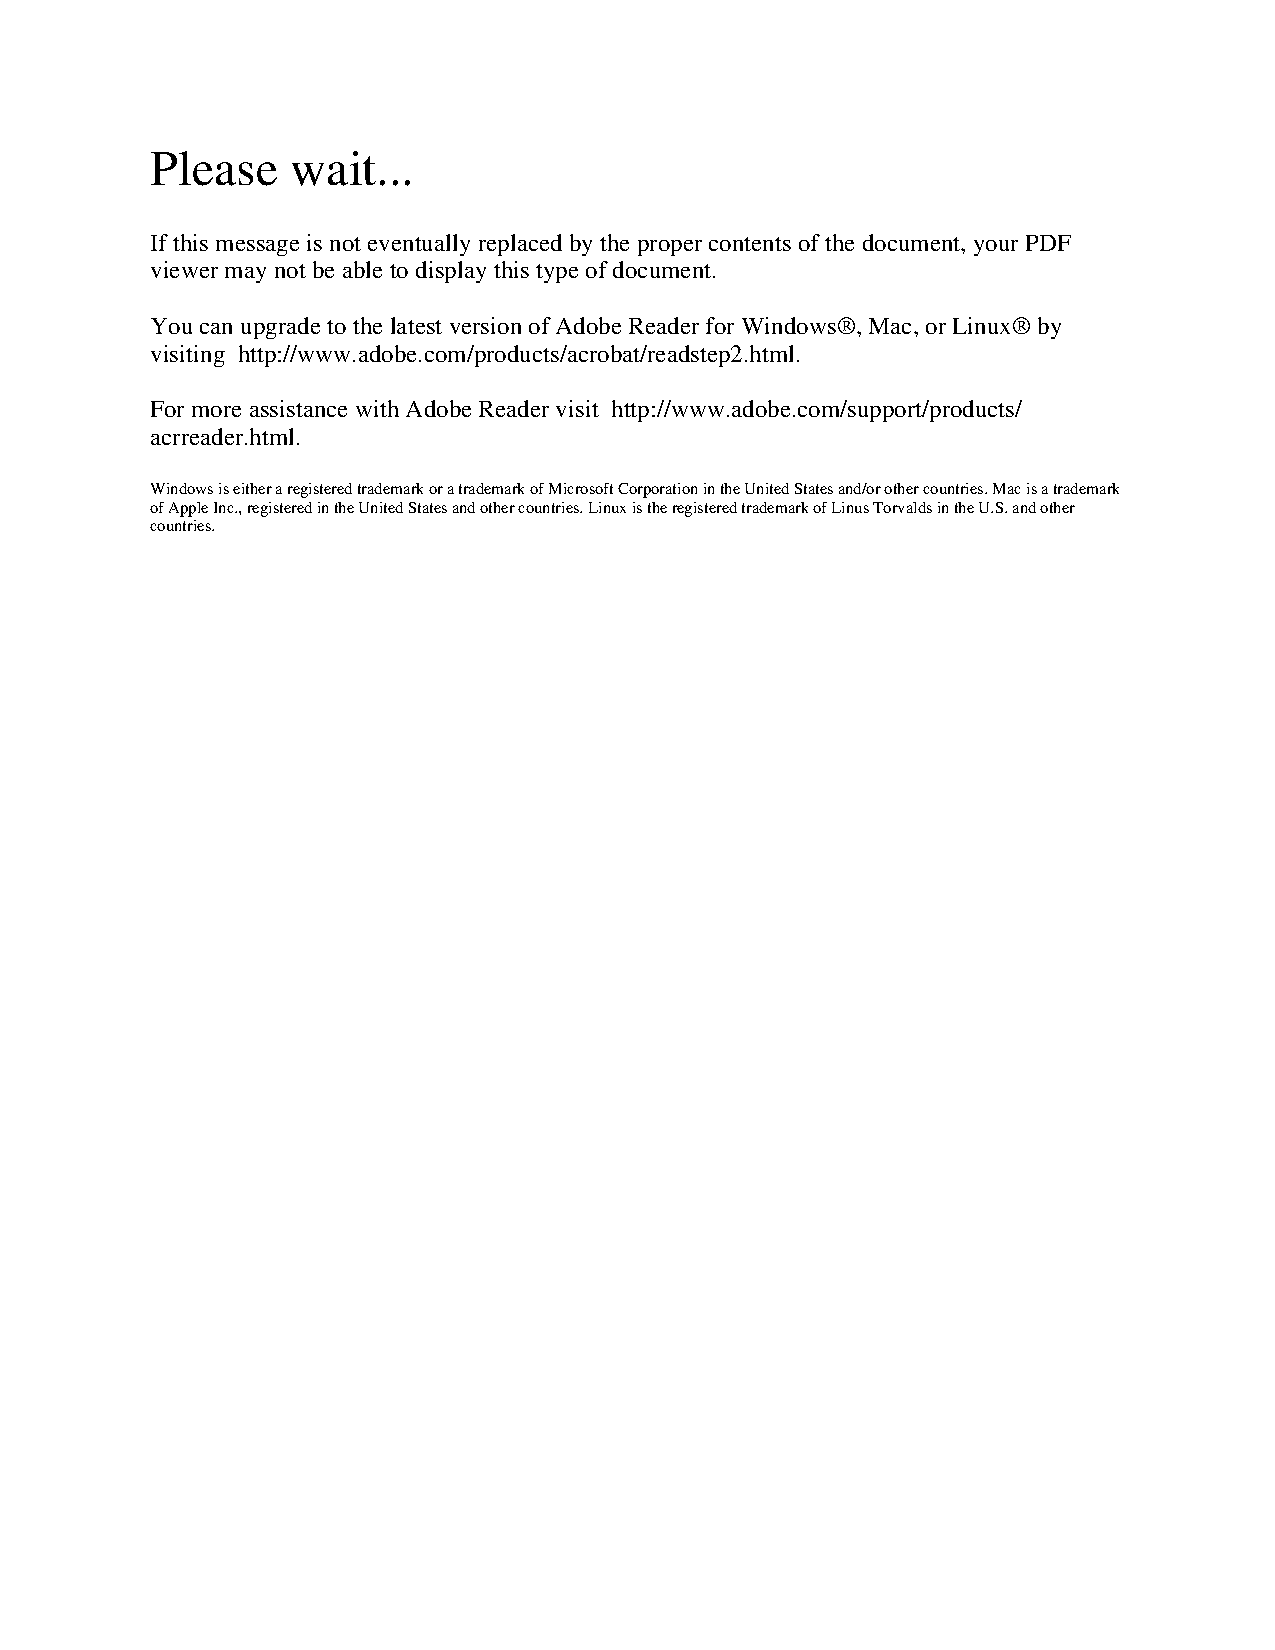
\includepdf{confirmation_en.pdf}

% IMPORTANT
% you MUST include the ETH declaration of originality here; it is available for download on the course website or at http://www.ethz.ch/faculty/exams/plagiarism/index_EN; it can be printed as pdf and should be filled out in handwriting


\newpage 
\paragraph*{
\centerline{\large{Abstract}}\newline
}
This paper is the final result of the course {\sc Modeling Social Systems with MATLAB} which aimed to offer an insight into the MATLAB programming language and to use said language to model social systems with various different approaches. The timeframe of the course is one semester.\\
In this paper we will try to show how to replicate the behaviour of desert ants in a MATLAB simulation. Furthermore we will discuss our results and compare them to experimental results obtained by biologists.


%%%%%%%%%% Table of content %%%%%%%%%%%%%%%%%

\tableofcontents

\newpage

%%%%%%%%%%%%%%%%%%%%%%%%%%%%%%%%%%%%%%%

\section{Individual contributions}
The whole project was done in a cooperative manner.
\newpage

\section{Introduction and Motivations}
We think ants are exciting animals because – despite their small body mass and therefore small brain – they form very huge and complex social structures. Very large numbers of them work together efficiently like one body. This requires a high level of coordination. We have already seen some videos which show the great achievements of ant colonies in building and hunting. Now we found out about their navigation abilities and are curious to learn how ants are able to cover extreme distances. The human being would definitely get lost when trying to journey this far in the desert without GPS or any other form of modern help, so one of our main goals will be to find out how ants can master this difficult task.

Ants have been subject of modern research since 1848, the motivations were often interest in their instincts, society and of course the hope to learn from them. Studies in ant movement became even more compelling when scientists started to look for algorithms that solve such fundamental tasks like finding the shortest way in a graph (Graph Theory). The class of ant colony optimization algorithms was introduced 1992 and has since been a field of active study.

However, those algorithms are using the behaviour of forest ants of the western hemisphere, which is not similar to the behaviour of desert in terms of choosing a good path and finding food. Since we are studying desert ants we had to take a different approach. Desert ants rely much more heavily on the few landmarks they find in their environment and less on pheromone tracks other ants have laid out before them, like forest ants do. Also they make use of a path-integrator with which they are able to track their position in reference to where they started the journey, most likely the nest.\\
Results of interest are: 
\begin{itemize}
\item How optimized is navigation by vectors 
\item What is the most energy-consuming task
\item Out of which states is it possible for the ant to find the nest (e.g. dropping the ant somewhere else, outside of her regular path etc.)
\item How well does the ant learn in the course of repeated journey towards the food and back
\end{itemize}
Of course we were as well motivated to improve our knowledge of MATLAB\texttrademark.
\newpage

\section{Description of the Model}

\begin{figure}[h]
	\centering
	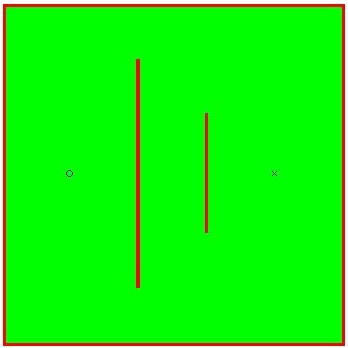
\includegraphics[scale=0.6]{../code/landscape.jpg}
	\caption[Sample Landscape]{Example of simple Landscape: obstacles red, feeder and nest are marked with x and o}
\end{figure}
\newpage

\section{Implementation}

\begin{figure}
	\centering
	\subfloat[Original Image]{\label{fig:original}\includegraphics[scale=0.4]{../code/map.png}
\end{figure}
\newpage

\section{Simulation Results and Discussion}
\newpage

\section{Summary and Outlook}
\newpage



\appendix
\section{Research Plan}

Group Name: The Anteaters Are Back\\
Group participants names: Wolf Vollprecht, Georg Wiedebach

\subsection*{General Introduction}

We think ants are exciting animals because – despite their small body mass and therefore small brain – they form very huge and complex social structures. Very large numbers of them work together efficently like one body. This requires a high level of coordination. We have already seen some videos which show the great achievngs of ant colonies in building and hunting. Now we found out about their naviagion abilities and are curious to learn how ants are able to cover extreme (in comparison to their own body size) distances. The human being would definitely get lost when trying to jurney this far in the desert wthout GPS or any other form of modern help, so one of our main goals will be to find out how ants can master this difficult task.

Ants have been subject of modern research since 1848, the motivations were often interest in their instincts, society and of couse the hope to learn from them. Studies in ant movement became even more compelling when scientists started to look for algorithms that solve such fundamental tasks like finding the shortest way in a graph (Graph Theorie). The class of ant colony optimization algorithms was introduced 1992 and has since been a field of active study.

\subsection*{Fundamental Questions}
\begin{enumerate}
\item How does ant movement and navigation work in challenging environments such as the desert?
\item Is ant communication connected to ant navigation?
\item Which mechanisms and factors influence ant movement?
\item Are there different strategies to find the shortest/safest etc. path?
\item How can we describe ant paths in mathematical terms?
\item How efficient are our mathematical models of the real ant behaviour?
\item How does our finding apply to the real world?
\end{enumerate}

We would like to create a model of desert ant behaviour. This will include their search for food, their returning to the nest and their orientation with global and local vectors. Also we will see how close our algorithms are to real ant movement. Therefore we want to simulate the experiments described in the papers. Our model should be able to deal with different numbers of landmarks, obstacles and starting points. We would like to give our ants the ability to learn and improve their efficency when searching and finding food. Of course there will be some simplifications we eventually will have to deal with: Such as ... will be updated during work on the simulation.

\subsection*{Expected Results}

We expect our simulation to be able to find short paths from Point A to desired positon B (i.e. feeder, nest) and back. We will try to be as cose to nature as possible and hope to be able to recreate some of the experimantal results given. Some results we consider particulary interesting are avoiding obstacles on returning home or finding a way to the nest after being deffered to a place where our ant has a non-fitting global vector. Of course we hope that there are already some good mathematical models available on ant movement, because these animals are topic of research for a long time already.
\\\\
The evolution may have taught ants a lot of useful tricks and methods to survive in environmets like the desert. Probably there are more ways to orientate than only by landmarks. Ants may have similar ways to find out their geographic orientation like pigeons, or use the sun as a fix-point. We are curious to find out more about that.

\section{Program Code}

\subsection{main.m}
\lstinputlisting{../code/main.m}
\subsection{simulation.m}
\lstinputlisting{../code/simulation.m}
\subsection{landscape.m}
\lstinputlisting{../code/landscape.m}
\subsection{ant.m}
\lstinputlisting{../code/ant.m}
\section{References}
\bibliographystyle{plain}
\bibliography{ant_behaviour_paper}
\listoffigures
\end{document} 